\chapter{Referencial teórico}
Neste capítulo, serão apresentados alguns conceitos importantes para a melhor compreensão do tema abordado por este projeto. O capítulo de referencial teórico foi organizado em dois escopos, um mais voltado à bibliografia investigada no domínio da Robótica Educacional e outro mais voltado à Engenharia de Software.
\section{Robótica educacional}
O uso dos robôs pelos seres humanos é datado de antes de Cristo, mas a definição da palavra robótica é recente. A robótica como instrumento de ensino está tomando força nos últimos anos, e vem apoiando muitos educadores na tarefa de fazer o aluno se sentir mais atraído pelo conteúdo, e aprender através de observações e manipulações. A seguir é abordado brevemente a história da robótica, bem como sua definição, seu uso no âmbito educacional e os fundamentos da robótica móvel. 
\subsection{Perspectiva histórica da robótica}
Os robôs são máquinas que podem substituir o homem na execução das tarefas, e consequentemente, destinados a melhorar a produção e a qualidade de vida \apud{antonio1997fundamentos}{santos2002robotica}. Desde os primórdios, o homem sente-se  atraído por esse mundo das máquinas, como os antigos Egípcios que adicionaram braços mecânicos às estátuas de seus deuses para serem operados por sarcedotes; e os Gregos que construíram estátuas movidas hidraulicamente; e os Chineses que entre os séculos XVIII e XIX contruíram bonecas que transportavam chá \cite{santos2002robotica}.
Os autômatos projetados pelos Gregos tinham uma função mais estética e contemplativa, já os projetados pelos Árabes tinham funcionalidade, deixando a par preocupações estéticas e de entretenimento \cite{santos2002robotica}.

É perceptível que os homens, há muitos séculos, utilizam os robôs, mas sem o conhecimento da palavra, que foi divulgada a primeira vez em 1921, pelo checoslovaco Karel Capek, no seu romance \textit{Rossum's Universal Robots}. Esse autor descreveu os robôs como máquinas com braços trabalhando duas vezes mais que os humanos, de forma incansável, eficiente e obediente, mas que se tornariam malévolos e dominariam o mundo \cite{santos2002robotica}. Porém em 1950, Isaac Asimov defendeu, em sua obra literária \textit{I Robot}, que a contrução de robôs seguiria uma linha positiva e benéfica \apud{nof1999handbook}{santos2002robotica}, concebendo-os como autômatos de aparência humana mas desprovidos de sentimentos \cite{santos2002robotica}.
Asimov, em sua obra, fala sobre a inteligência dos robôs de acordo com as seguintes leis da robótica \cite{santos2002robotica}:
\begin{itemize}
\item 1ª Lei: Um robô não pode prejudicar um ser humano, ou quando inativo, deixar um ser humano exposto ao perigo;
\item 2ª Lei: Um robô deve obedecer às ordens dadas pelo ser humano, exceto se tais ordens  estiverem em contradição com a 1ª Lei.
\item 3ª Lei: Um robô deve proteger a sua própria existência desde que essa proteção não entre em conflito com a 1ª e a 2ª Leis.
\end{itemize}
Dessa forma, Asimov popularizou o termo robô e idealizou as três leis fundamentais da robótica \cite{de2008utilizaccao}.

\subsection{Definição de robô e robótica}
A Divisão Internacional de Robótica da Sociedade de Engenharia de Manufatura define um robô como sendo um manipulador reprogramável, multifunções, utilizado para deslocar outros materias ou objetos específicos através da programação de movimentos \cite{de2008utilizaccao}. Um computador é manipulado pelo homem, logo não é considerado um robô, pois um robô é um mecanismo inteligente que funciona de forma autônoma \cite{curcio2008instituto}.
	
\cite{de2006robotica} definem a robótica como: 
\begin{citacao}
a ligação inteligente entre a percepção e a ação. Trabalhar em Robótica significa estudar, projetar e implementar sistemas ou dispositivos que, com a utilização de percepção e de certo grau de “inteligência”, sejam úteis na realização de uma determinada tarefa, pré-definida ou não, que envolva interação física entre o sistema (ou dispositivo) e o meio onde a tarefa está sendo realizada.
\end{citacao}
Porém, uma definição mais formal para o termo robótica seria "uma ciência da engenharia aplicada, tida como uma combinação da tecnologia de máquinas operatrizes e ciência da computação" \apud{groover1989robotica}{redel2004implementaccao}. Assim, a robótica envolve várias disciplinas como engenharia mecânica, elétrica, inteligência artificial e utiliza o robô como principal instrumento \cite{curcio2008instituto}.
Os robôs podem ser categorizados em primeira, segunda e terceira geração, sendo progressivamente mais inteligentes \apud{antonio1997fundamentos}{santos2002robotica}.
\begin{itemize}
\item Primeira geração: A única função inteligente desses robôs é a apredizagem de uma sequência de ações de manipulação, coordenadas por um operador humano usando uma unidade de comando. Os robôs dessa geração repetem sistematicamente as tarefas e ignoram possíveis alterações no meio externo, causando restrições no seu uso, como posicionamento no espaço, relacionamento com outras máquinas e a segurança das pessoas que ficam próximas ao robô. 
\item Segunda geração: esses robôs tiveram a adição de um processador à sua configuração, possibilitando a adaptabilidade ao ambiente, mesmo que de forma mínima, com utilização de sensores para auxiliar na localização, detecção de esforços e adaptação de seus movimentos às informações coletadas. Geralmente a área de atuação destes robôs está ligada à manufatura autômata.
\item Terceira geração: é uma versão mais recente dos robôs, na qual é incorporado à sua configuração, processadores múltiplos em que, cada operação em sicronia desempenha uma tarefa diferente, tornando um mesmo robô multitarefas.	 
\end{itemize}

\subsection{Robótica como instrumento educacional}
A róbótica educacional é um meio de inserir a tecnologia no meio educativo como forma de aprendizado, oferencendo aos alunos uma oportunidade de vivenciarem experiências semelhentes às que vivem na vida real.
\subsubsection{Teorias de aprendizagens}
A teoria de aprendizado que fundamentou a róbotica educacional foi a construcionista, criada por Seymour Papert, baseada na teoria construtivista criada por Jean Piaget. Dentre as várias teorias de aprendizado existentes, algumas são brevemente descritas a seguir, segundo \cite{zilli2004robotica}.
\begin{enumerate}
\item \textbf{Teoria das inteligências múltiplas:} Howard Gardner, professor e psicólogo da \textit{Harvard Graduate School of Education}, dedicou-se, desde a década de 80, ao estudo das capacidades simbólicas em crianças com QI normal e alto, desenvolvendo o que ele chamou de "inteligências múltiplas". Essas podem ser vista como contendo três princípios fundamentais:
\begin{itemize}
\item A inteligência não é algo que pode ser visto como tendo múltiplas habilidades. Existem múltiplas inteligências, cada uma com habilidades distintas entre si.
\item  As inteligências são interdependentes. Logo, caso seja avaliada a competência de uma pessoa em uma área, esta avaliação não servirá para outras áreas.
\item Apesar de serem interdependentes, as inteligências podem sim trabalhar em conjunto; caso contrário nada seria feito e nenhum problema seria resolvido.
\end{itemize}
Gardner identificou essas inteligências distintas e classificou da seguinte forma:
\begin{itemize}
\item Inteligência linguística: é relacionada à habilidade da pessoa em produzir a liguagem escrita e falada.
\item Inteligência lógico-matemática: é relacionada à habilidade para explorar relações, categorias e padrões, por meio da manipulação de objetos ou símbolos, e à habilidade de resolver problemas por meio do raciocínio.
\item Inteligência musical: é relacionada, como o próprio nome já diz, ao reconhecimento da estrutura musical, à sensibilidade dos sons, à criação de melodias e ritmos, à percepção das qualidades dos tons e à habilidade para tocar instrumentos.
\item Inteligência espacial: é relacionada à habilidade do indivíduo de visualizar um objeto e ter uma percepção acurada de diferentes ângulos, relações de espaço, dentre outros.
\item Inteligência cinestésica: é representada pela capacidade de manipular objetos habilmente e controlar os movimentos do corpo.
\item Inteligência interpessoal: é relacionada à capacidade de diferenciar e dar uma resposta aos estados de humor, temperamentos, desejos e motivações das outras pessoas.
\item Inteligência intrapessoal: é relacionada à habilidade para ter acesso aos próprios sentimentos, aos estados interiores do ser, e saber utilizá-los na solução de problemas pessoais. 
\end{itemize}
Segundo Gardner, a escola valoriza mais a inteligência linguística e a lógico-matemática, e o uso do computador pode colaborar para o amadurecimento das outras inteligências, por ser uma ferramenta adaptável às mais diversas formas de uso.

\item \textbf{Teoria do ensino por competências:} Philippe Perrenoud, professor e sociólogo suiço, é referência para diversos educadores com suas idéias pioneiras e vanguardistas sobre profissionalização de professores e avaliação de alunos. Perrenoud afirma que "a trilogia das habilidades de ler, escrever, contar, que fundou a escolaridade obrigatória no século XIX não está mais a altura das exigências da nossa época". Assim, Perrenoud propôs o ensino por competências que considera que os saberes são ferramentas para a ação e que se aprende a usá-los. O Centro de Referência Educacional elencou dez competências que devem ser trabalhadas pela escola: 
\begin{itemize}
\item Respeitar as identidades e as diferenças;
\item Utilizar-se das linguagens como meio de expressão, comunicação e informação;
\item Inter-relacionar pensamentos, ideias e conceitos;
\item Desenvolver o pensamento crítico e flexível e a autonomia intelectual;
\item Adquirir, avaliar e transmitir informações;
\item Compreender os princípios das tecnologias e suas relações integradoras;
\item Entender e ampliar fundamentos científicos e tecnológicos;
\item Desenvolver a criatividade; 
\item Saber conviver em grupo; 
\item Aprender a aprender.
\end{itemize} 

\item \textbf{Teoria do construtivismo:} O suiço Jean Piaget estudou como o aprendiz passa de um estado de menor conhecimento para outro de maior conhecimento, e desenvolveu a teoria do construtivismo que foca no conhecimento científico na perspectiva do indivíduo que aprende. Nessa teoria, o sujeito é um ser ativo que estabelece relação de troca com o meio-objeto, relações essas que devem ser vivenciadas e significativa. Assim, o indivíduo incorpora novas informações, que passa a tornar parte do conhecimento. Segundo \cite{zilli2004robotica}, 

\begin{citacao}
O construtivismo defende que o conhecimento não é uma cópia da realidade, mas sim
uma construção do ser humano em conseqüência da sua interação com o ambiente e resultado de suas disposições internas.
\end{citacao} 

Piaget classifica os períodos de inteligência em estágios, organizados do nascimento até a fase adulta. Esses estágios indicam saltos bruscos nas capacidades do indivíduo, pois as capacidades cognitivas sofrem uma forte reestruturação.

\item \textbf{Teoria do construcionismo:} Seymour Papert, psicólogo do Laboratório de Inteligência Artificial do MIT, adaptou os princípios do construtivismo definido por Piaget e criou a teoria construcionista, que considera o computador como uma ferramenta para a construção do conhecimento e desenvolvimento do aluno. Duas ideias principais sobre a construção do conhecimento fazem com que o construcionismo se diferencie do construtivismo:
\begin{itemize}
\item O aprendiz é quem constrói o conhecimento, através das coisas que faz;
\item O aprendiz constrói algo do seu interesse e que o motiva. 
\end{itemize} 
Segundo Papert, a criança aprende de forma mais eficaz quando, por ela mesma, atinge o conhecimento específico de que precisa. O contrucionismo tem como meta ensinar de forma a produzir o maior conhecimento possível com o mínimo de ensino.
\end{enumerate}

\subsubsection{Conceito da robótica educacional}
\cite{maisonnette2002utilizaccao} define róbotica como sendo
\begin{citacao}
o controle de mecanismos eletro-eletrônicos através de um computador, 
transformando-o em uma máquina capaz de interagir com o meio ambiente e executar 
ações decididas por um programa criado pelo programador a partir destas interações. 
\end{citacao}
\cite{maisonnette2002utilizaccao} também afirma que a robótica educacional é a aplicação dessa tecnologia como mais uma ferramenta de ensino para que os alunos vivenciem de forma real o que estudam, tendo a oportunidade de propor e solucionar problemas difíceis ao invés de apenas observar a solução.
Através da robótica educacional, os alunos podem explorar ideias e descobrir novos caminhos na aplicação de conceitos que aprendem em sala de aula. Dessa forma, adquirem a capacidade de produzir hipóteses, averiguar soluções, estabelecer relações e inferir conclusões \cite{benitti2009experimentaccao}.
Além de benéfico ao aluno, a robótica educacional colabora com o professor no ensino de muitos conceitos teóricos de difícil compreensão, motivando o aluno a observar, abstrair e inventar. O conhecimento adquirido através de observação, abstração e do esforço do aluno tem muito mais significado para ele, e se adapta melhor às suas estruturas mentais \cite{zilli2004robotica}.

\subsubsection{Objetivos da robótica educacional}
Segundo \cite{zilli2004robotica}, além de propiciar o conhecimento da tecnologia atual, a robótica educacional pode desenvolver as seguintes competências:
\begin{itemize}
\item raciocínio lógico;
\item habilidades manuais e estéticas;
\item relações inter e intrapessoais;
\item utilização dos conceitos aprendidos em diversas áreas do conhecimento para o desenvolvimento de projetos;
\item investigação e compreensão;
\item representação e comunicação;
\item trabalho com pesquisa;
\item resolução de problemas por meio de tentativa e erro;
\item aplicação das teorias às atividades concretas;
\item utilização da criatividade em diversas situações, e
\item capacidade crítica.
\end{itemize}

\cite{zilli2004robotica} também apresentam uma classificação dos objetivos da robótica educacional:
\begin{itemize}
\item Objetivos Gerais
\begin{itemize}
\item Contruir maquetes que utilizem lâmpadas, motores e sensores;
\item Trabalhar conceitos de desenho, física, álgebra e geometria;
\item Conhecer e aplicar princípios de eletrônica digital, e
\item Construir ou adaptar elementos dinâmicos como engrenagens, redutores de velocidade de motores, entre outros.
\end{itemize}
\item Objetivos Psicomotores
\begin{itemize}
\item Desenvolver a motricidade fina;
\item Proporcionar a formação de habilidades manuais;
\item Desenvolver a concentração e observação, e
\item Motivar a precisão de seus projetos.
\end{itemize}
\item Objetivos Cognitivos
\begin{itemize}
\item Estimular a aplicação das teorias formuladas às atividades concretas;
\item Desenvolver a criatividade dos alunos;
\item Analisar e entender o funcionamento dos mais diversos mecanismos físicos;
\item Ser capaz de organizar idéias a partir de uma lógica mais sofisticada de pensamento;
\item Selecionar elementos que melhor se adequem à resolução dos projetos;
\item Reforçar conceitos de matemática e geometria;
\item Desenvolver noções de proporcionalidade;
\item Desenvolver noções topológicas;
\item Reforçar a aprendizagem da liguagem Logo;
\item Introduzir conceitos de robótica;
\item Levar à descoberta de conceitos de física de forma intuitiva;
\item Utilizar conceitos aprendidos em outras áreas do conhecimento para o desenvolvimento de um projeto, e
\item Proporcionar a curiosidade pela investigação levando ao desenvolvimento intelectual do aluno.
\end{itemize}
\item Objetivos Afetivos
\begin{itemize}
\item Promover atividades que geram a cooperação em trabalhos em grupo;
\item Estimular o crescimento individual através da troca de projetos e ideias;
\item Garantir que o aluno se sinta interessado em participar de discussões e trabalhos em grupo;
\item Desenvolver o senso de responsabilidade;
\item Despertar a curiosidade;
\item Motivar o trabalho de pesquisa;
\item Desenvolver a autoconfiaça e a auto-estima, e
\item Possibilitar a resolução de problemas por meio de erros e acertos.
\end{itemize}
\end{itemize}

\subsection{Fundamentos da robótica móvel}
O foco da robótica vem se modificando ao longo dos anos. Tempos atrás, os braços mecânicos, também chamados de manipuladores, tinham um maior destaque junto a mídia e a sociedade em geral \cite{wolf2009robotica} sendo até um dos principais fatores para a Revolução Industrial. Nos tempos atuais, o destaque é a robótica móvel, que trata de máquinas capazes de se movimentar de forma independente, podendo ser terrestre, aquático, voador ou até espacial \apud{vieira2005controle}{rinconframework}, movidos por rodas, esteiras, patas, hélices, dentre outros. 

Segundo \cite{wolf2009robotica} os Robôs Móveis Autônomos (RMA) possuem como características fundamentais

\begin{citacao}
as capacidades de locomoção e de operação de modo semi ou 
completamente autônomo. Também deve ser considerado que maiores níveis de 
autonomia serão alcançados somente à medida que o robô passe a integrar outros 
aspectos considerados da maior importância, como: \textit{capacidade de percepção} (sensores que conseguem “ler” o ambiente onde ele atua), \textit{capacidade de agir} (atuadores e motores capazes de produzir ações, tais como o deslocamento do robô no ambiente), \textit{robustez e inteligência} (capacidade de lidar com as mais diversas situações, de modo a resolver e executar tarefas por mais complexas que sejam). 
\end{citacao}

O termo Controle Robótico Inteligente é referente ao uso de técnicas de planejamento e controle para a navegação e operação autônoma dos robôs, que permitem que os RMAs tenham a capacidade de executar as mais diversas e complexas tarefas. Esse controle inteligente é possível devido ao uso de diversos sensores e atuadores que combinados conferem ao robô a possibilidade de planejar e realizar o acionamento de seus dispositivos de modo a executar a ação desejada. Alguns sensores e atuadores para robôs móveis são listados, respectivamente, nas Figuras \ref{sensores} e \ref{atuadores}, a seguir apresentadas.

\FloatBarrier
\begin{figure}[!h]
\centering
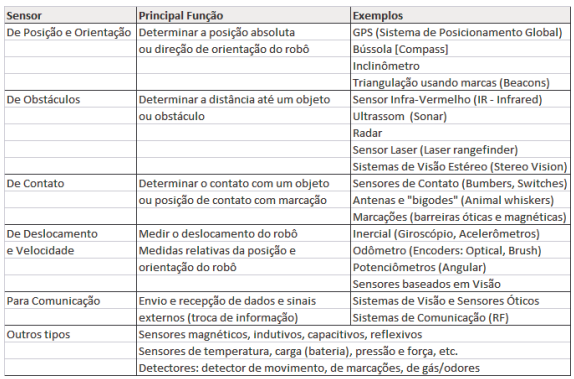
\includegraphics[keepaspectratio=true,scale=0.7]{figuras/sensoresRobosMoveis.png}
\caption{Tipos de sensores para robôs móveis \cite{wolf2009robotica}}
\label{sensores}
\end{figure}

\FloatBarrier
\begin{figure}[!h]
\centering
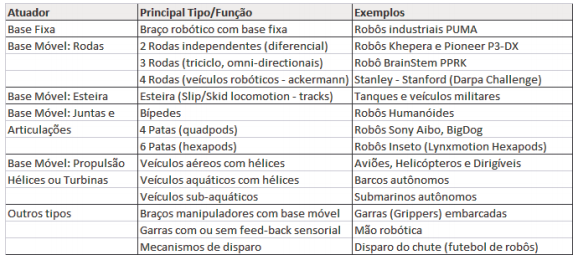
\includegraphics[keepaspectratio=true,scale=0.7]{figuras/atuadoresRobosMoveis.png}
\caption{Tipos de atuadores para robôs móveis \cite{wolf2009robotica}}
\label{atuadores}
\end{figure}

Os sensores conferem ao robô uma visão parcial, incompleta e sujeita a erros, sendo tarefa do controle inteligente adquirir, unificar e tratar as informações providas pelos sensores. Os comandos dos atuadores também são imprecisos, pois estes estão sujeitos a erros de posicionamento do robô e acionamento dos motores, além das forças externas, como fricção, gravidade, colisão com obstáculos, derrapagem de rodas, dentre outros. Nesse contexto, cabe ao controle inteligente prover técnicas que permitam contornar estes cenários, corrigindo os erros de modo que as tarefas do robô sejam executadas corretamente \cite{wolf2009robotica}.

Um projeto de sistema de controle de robô deve levar em conta uma série de quesitos como: i)tipo de tarefa do robô; ii)tipo e precisão dos sensores embarcados, e iii)tipo e precisão dos atuadores. Além de adotar uma arquitetura específica de controle que seja capaz de realizar algumas tarefas específicas ou, no melhor dos casos, todas as tarefas, sendo elas: i) fusão de sensores; ii)desviar de obstáculos; iii)auto-localização; iv)mapeamento do ambiente v)planejamento de trajetórias; vi)planejamento de ações; vii)navegação robótica e viii)interação e comunicação. O detalhamento de cada tópico pode ser conferido na íntegra em \cite{wolf2009robotica}. 
Para que essas tarefas sejam planejadas e executadas gerenciando todos os dispositivos embarcados no robô, é necessário fazer o uso das arquiteturas computacionais de controle de robôs móveis autômatos. Essas arquiteturas computacionais são relativas à percepção, raciocínio/decisão e ação em relação ao ambiente \cite{wolf2009robotica}. Dentre os diversos tipos de arquiteturas computacionais, as mais conhecidas e reconhecidas são controle reativo, controle deliberativo, controle hierárquico e controle híbrido. Cada uma delas é descrita a seguir.

\subsubsection{Controle reativo}
O controle reativo consiste em um sistema de reação sensorial-motora que considera apenas as leituras sensoriais realizadas no presente para fins de tomada de decisão e geração de comandos de ação \cite{wolf2009robotica}. Esse tipo de arquitetura computacional tem por objetivo possibilitar a implementação de sistemas de controle com rápida resposta a um grande número de ocorrências ou situações de ambiente, permitindo que os robôs atuem em ambientes dinâmicos, devido a simplicidade no tratamento das informações sensoriais e a forma direta pela qual a percepção está associada com a ação \apud{grassi2006arquitetura}{industriais2009sistema}. 

	\cite{wolf2009robotica} defendem que o sistema reativo é muito útil para implementar comportamentos.
\begin{citacao}
Um sistema reativo é bastante útil para implementar comportamentos elementares como: desviar de obstáculos (\textit{avoid collision behaviour}: reage a presença de um obstáculo), seguir um objeto (\textit{wall-following behaviour}: acompanhar um elemento guia) e seguir uma fonte luminosa (\textit{phototaxis behaviour}: mover em direção a uma fonte de luz). 
\end{citacao}

\subsubsection{Controle deliberativo}
A arquitetura deliberativa consiste em aplicar um mecanismo de planejamento e tomada de decisão que estabeleça um plano prévio de execução de uma sequência de ações, baseado no modelo interno de conhecimento do mundo que o robô possui. Esse conhecimento prévio do mundo confere ao robô a possibilidade de otimizar o desempenho em relação ao modelo interno. 

O robô pode ter seu modelo interno representado de duas formas diferentes: simbólica e geométrica. O modelo simbólico é baseado em lógica utilizando, muitas vezes, a inteligência artificial. Já no modelo geométrico o mundo é representado espacialmente, por espaços livres e com obstáculos \cite{industriais2009sistema}.

Tendo em vista que o robô possui esse modelo interno de mundo previamente estabelecido, ele possui limitações quando colocado em um mundo dinâmico, pois será necessário reconhecer o novo obstáculo, acrescentar ao seu modelo e reestabelecer o plano de execução \cite{industriais2009sistema}. Devido a essa limitação, \cite{wolf2009robotica} dizem que o melhor seria a combinação dos modelos reativos e deliberativos, assim o robô teria capacidade de reação e de planejamento de tarefas complexas. 

\subsubsection{Controle hierárquico}
O controle hierárquico consiste na combinação de múltiplos módulos de controle (reativo e/ou deliberativo) dispostos em forma hierárquica, podendo ser com decomposição vertical ou horizontal para definir um esquema de prioridades em relação às múltiplas camadas do sistema \cite{wolf2009robotica}.

O controle hierárquico com decomposição vertical possui os módulos de controle reativo dispostos de forma vertical, mantendo a prioridade de baixo para cima, sendo a camada mais baixa a mais prioritária. Um exemplo de uso desse modelo é quando a ação de desviar de um obstáculo, que está mais baixa, tem prioridade em relação a ação de seguir em frente, que está mais acima.

O controle hierárquico com decomposição horizontal é adotado para controle de módulos deliberativos, implementando um \textit{"pipeline"} que decompõe as funções em camadas executadas em cascata, formando uma linha de ação horizontal. Um exemplo desse modelo é o tipo Sense-Model-Plan-Act (SMPA) que possui um longo ciclo de resposta ao estímulo de entrada devido as suas quatro camadas horizontais que serão executadas em cascata para cada estímulo.

\subsubsection{Controle híbrido}
A arquitetura de controle híbrido nada mais é do que um controle reativo sendo planejado por um controle deliberativo. Inicialmente, é realizado um plano de execução pelo módulo deliberativo. Depois de pronto, o plano é executado por um módulo reativo de maior prioridade, o qual pode intervir nesse plano quando encontra algum obstáculo em meio à execução das ações. Nesse controle, pode-se ainda ter um módulo de auto-localização que monitora constantemente a posição atual do robô e a corrige, se necessário.

Este tipo de arquitetura é uma das mais sofisticadas e adotadas na implementação dos sistemas de controle dos robôs móveis autônomos modernos, devido a sua eficiência em atingir os objetivos do robô. 

\section{Engenharia de software}
O estudo da robótica na Universidade tem um foco considerável na inteligência artificial, e uma das áreas desta é a otimização. A seguir são brevemente descritos os dois algoritmos de otimização abordados por este trabalho, o algoritmo guloso e a programação dinâmica, bem como o paradigma lógico, também tema deste trabalho.
\subsection{Algoritmo guloso}
Os algoritmos gulosos tomam uma decisão levando em consideração apenas a informação disponível no dado momento, sem levar em conta as consequências da decisão, nunca reconsiderando uma decisão já tomada. Dessa forma, o algoritmo guloso toma uma decisão ótima naquele momento (decisão ótima local), e espera que essa decisão seja também a ótima global \cite{anderson2004}.
\subsubsection{Características do algoritmo guloso}
Segundo \cite{anderson2004}, os problemas e os algoritmos gulosos que os resolvem são caracterizados pelos itens a seguir.
\begin{itemize}
\item Para que exista uma solução ótima de um problema deve existir um conjunto de candidatos;
\item Ao executar um algoritmo guloso dois conjuntos são criados: um que contêm os elementos que foram analisados e rejeitados e outro os elementos que foram analisados e escolhidos;
\item Um algoritmo guloso contêm quatro funções: 
\begin{itemize}
\item a primeira avalia se o conjunto candidato produz uma solução para o problema; 
\item a segunda verifica a viabilidade do conjunto de candidatos, ou seja, se é possível acrescentar mais candidatos a esse conjunto; 
\item a terceira função, chamada de função seleção, avalia qual dos candidatos restantes é o melhor para ser acrescentado no conjunto; 
\item a quarta e última função, chamada função objetivo, retorna o valor da solução encontrada.
\end{itemize} 
\end{itemize}
É possivel dizer que um algoritmo guloso trabalha da seguinte forma: inicialmente contém um conjunto S que está vazio, ou seja, nenhum candidato foi escolhido. A cada passo a função seleção é utilizada para determinar qual o melhor candidato. Se o elemento analisado não é viável, ignora-se o termo que está sendo avaliado no momento. Se for viável, adiciona o elemento ao conjunto S. O elemento avaliado, sendo ele aceito ou rejeitado, será avaliado apenas uma vez, não havendo reconsiderações. A cada vez que o conjunto de candidatos escolhidos (S) é ampliado, é verificado se a solução do problema foi obtida \cite{anderson2004}.  
\subsubsection{Elementos da estratégia gulosa}
Como exposto, a estratégia utilizada pelo algoritmo guloso para encontrar a solução ótima do problema em questão é em cada passo escolher a solução que parece ser ótima naquele momento. Nem sempre uma estratégia gulosa é capaz de chegar à solução de um problema, mesmo esta existindo. Existem duas características que podem indicar se o problema pode ou não ser resolvido através de uma estratégia gulosa.
\begin{itemize}
\item \textbf{Propriedade da escolha gulosa:} Segundo a propriedade da escolha gulosa, uma solução globalmente ótima pode ser alcançada escolhendo uma solução localmente ótima. Para se provar que uma escolha localmente ótima em cada um dos passos irá levar a uma solução ótima é necessário examinar uma solução ótima global para algum subproblema. Posteriormente, deve-se mostrar que essa solução pode ser modificada em uma solução gulosa. Tal estratégia irá resultar em um subproblema menor, mas similiar.
\item \textbf{Subestrutura ótima:} Esta característica também é importante quando se utiliza a programação dinâmica, vide seção \ref{Programação dinâmica}. Um problema possui uma subestrutura ótima quando uma solução ótima para o problema contêm, dentro dela, soluções ótimas para os subproblemas.
\end{itemize}
\subsubsection{Fundamentos do algoritmo guloso}
A teoria de algoritmos gulosos envolve o conceito de matróide que por definição é um par (E,I) onde E é um conjuto finito e I $\subseteq 2^{E}$, que satisfaz os seguintes axiomas \cite{paulo2007cobertura}:
\begin{enumerate}[label=(\roman*)]
\item $\emptyset \in$ I;
\item Se X $\subseteq$ Y e Y $\in$ I, então X $\in$ I;
\item Se X, Y $\in$ I e |X| < |Y| então existe e $\in$ Y - X tal que X $\cup$ e $\in$ I.
\end{enumerate}
Esse tipo de estrutura não cobre todo tipo de problema que pode ser resolvido pelo algoritmo guloso, mas cobre muitos casos de interesse prático.

\textbf{Lema:} todo conjunto independente maximal em um matróide tem o mesmo tamanho. 
\textbf{Prova:}  Por contradição. Se existir dois conjuntos independentes maximais A e B e |A| < |B|, deve existir um elemento x $\in$ (B - A) tal que (A + x) $\in$ I. Isso contradiz o fato de que A é um conjunto maximal.

\subsection{Programação dinâmica} \label{Programação dinâmica}
A programação dinâmica, assim como os métodos de "dividir para conquistar", combina as soluções dos subproblemas para resolver um problema. Esses métodos particionam os problemas em subproblemas de forma que resolvendo os subproblemas, recursivamente, resolve-se o problema. Já a programação dinâmica aplica-se quando os subproblemas se particionam em subsubproblemas. Um algoritmo comum resolve repetidamente essas partições, trabalhando mais que o necessário. Em contrapartida, o algoritmo dinâmico resolve cada subsubproblema apenas uma vez, salvando o resultado em uma tabela, evitando calcular repetidas vezes o mesmo problema \cite{cormen2009introduction}.
Um problema pode ter várias soluções possíveis, cada uma com um valor, e a solução com o melhor valor (maior ou menor) é dita a solução ótima para o problema.
Segundo \cite{cormen2009introduction} para se desenvolver uma solução de programação dinâmica devem ser seguidos quatro passos:
\begin{itemize}
\item Caracterizar a estrutura de uma solução ótima;
\item Recursivamente definir o valor de uma solução ótima;
\item Calcular o valor de uma solução ideal, normalmente de forma ascendente, e
\item Construir uma solução ótima a partir de informações computadas. 
\end{itemize}
Os três primeiros itens formam a base de uma solução dinâmica. Mas, quando utilizar a programação dinâmica para resolver um problema? O primeiro passo para resolver um problema de otimização por programação dinâmica é caracterizar uma subestrutura ótima, sempre que um problema exibi-la. 
Para caracterizar o espaço de subproblemas, deve-se manter o espaço o mais simples possível e, em seguida, expandi-lo, se necessário. Uma subestrutura ótima varia entre os domínios de problema de duas formas:
\begin{enumerate}[label=(\roman*)]
\item quantos subproblemas uma solução ideal utiliza para o problema, e
\item quantas escolhas existem para determinar quais subproblemas usar em uma solução ótima.
\end{enumerate}
Ou seja, pode ser que um problema tenha apenas um subproblema (de tamanho n - i), mas deve-se considerar n escolhas para i, afim de determinar quais escolhas produzem uma solução ótima.

\subsubsection{\textit{Memoization} vs Iteração sobre subproblemas} 
A palavra \textit{memoization} vem do termo \textit{memoize} que deriva de um termo latim \textit{memorandum} que quer dizer relembrando. Essa é uma técnica \textit{top-down} que  armazena em uma tabela a solução de cada subsubproblema, evitando assim o retrabalho e aumentando a eficiência. Essa técnica utiliza um algoritmo recursivo.

A iteração sobre subproblemas é uma técnica \textit{buttom-up} que utiliza um algoritmo iterativo para calcular os subproblemas. Essa técnica começa a calcular do menor subproblema para o maior. 

\subsection{Paradigma lógico}
Os literais são fórmulas atômicas positivas ou negativas, que em conjunto formam uma cláusula. Um tipo de cláusula é a chamada cláusula de Horn (ou cláusula definitiva), onde cada cláusula tem no máximo um literal positivo. Essas cláusulas são utilizadas pela resolução SLD (Selection-rule driven Linear resolution for Definite clauses), que restringe o uso de literais para tornar as implementações mais eficientes. Essa resolução recebe como entrada um programa lógico P e uma consulta N, e efetua a resolução entre a consulta N e alguma regra de P. O ganho de eficiência vem do fato de que, para cada regra é possível a seleção de apenas um literal para a resolução com N \cite{rodrigues2010fundamentos}.
A programação lógica surgiu da aplicação da SLD no processamento da linguagem natural da  inteligência artificial, e esse processamento serviu como primeira aplicação e motivo imediato para o desenvolvimento do Prolog (Programation en Logique) \cite{rodrigues2010fundamentos}.
\subsubsection{Prolog}
O Prolog é uma linguagem de programação utilizada para resolver problemas que envolvam objetos e relações entre objetos. O termo objeto em Prolog não se refere a uma estrutura de dados que pode herdar variáveis e métodos de uma classe, mas se refere às coisas que podemos representar usando termos \cite{clocksin2003programming}.
Um programa Prolog consiste em um conjunto de cláusulas, onde cada cláusula ou é um fato sobre a informação dada ou uma regra sobre como a solução pode relacionar ou ser inferida a partir dos fatos dados \cite{clocksin2003programming}.
Segundo \cite{clocksin2003programming}, a programação em Prolog consiste em: 
\begin{itemize}
\item especificar algum fato sobre os objetos e seus relacionamentos;
\item definir algumas regras sobre objetos e seus relacionamentos, e
\item fazer perguntas sobre os objetos e seus relacionamentos.
\end{itemize}
O Prolog pode fazer muito mais do que apenas responder sim ou não às perguntas feitas, ele permite que um computador seja usado como um armazém de fatos e regras, fornecendo maneiras de se fazer inferências a partir de um fato ou outro e encontrar os valores das variáveis que levam a uma dedução lógica.
Algumas definições base da linguagem Prolog são descritas a seguir.
\begin{itemize}
\item \textbf{Fato:} um fato é a definição das relações entre os objetos. Para implementar essas definições, algumas regras devem ser seguidas i) os nomes de todas as relações e objetos devem começar com letra minúscula; ii) a relação é escrita primeiro seguida do(s) objeto(s) entre parênteses (caso tenha mais de um separar com vírgula); iii) um fato deve terminar com ponto-final. A relação entre os objetos é chamada de predicado, e os objetos da relação são chamados de argumentos.
\item \textbf{Questão:} a questão tem a escrita muito parecida com o fato, exceto que começa com um ponto de interrogação. Para cada pergunta feita ao interpretador de Prolog, ele irá procurar na sua base de conhecimento fatos ou regras que comprovem aquele questionamento. 
\item \textbf{Variáveis:} é um nome com letra maiúscula. Quando utilizado em uma pergunta, faz com que o intepretador de PROLOG procure na base de conhecimento um ou mais objetos que sejam equivalentes àquela variável. Como por exemplo, nessa base de conhecimento exitem três fatos: 

\lstset{language=Prolog}
\begin{lstlisting}
gosta(maria, pedro).
gosta(maria, joao). 
gosta(laura, joao).
\end{lstlisting}

Quando for perguntado ao prolog:
\lstset{language=Prolog}
\begin{lstlisting}
?- gosta(maria, X).
\end{lstlisting}

O interpretador Prolog responderá:
\lstset{language=Prolog}
\begin{lstlisting}
X = pedro;
X = joao.
\end{lstlisting}

\item \textbf{Conjunção:} é o operador vírgula (,) tendo função de "e". Quando utilizado na pergunta, por exemplo, o interpretador de Prolog procura na base de conhecimento fatos que comprovem as duas perguntas. Usando a base de conhecimento do item anterior, se perguntar ao interpretador de Prolog: 
\lstset{language=Prolog}
\begin{lstlisting}
?- gosta(maria, X) , gosta(laura, X).
\end{lstlisting}
ele responderá:
\lstset{language=Prolog}
\begin{lstlisting}
X = joao.
\end{lstlisting}
Para responder a esse questionamento, o interpretador de Prolog procura primeiramente qual o objeto que pode ser a variável X, achando inicialmente o argumento pedro. Em seguida, ele procura se existe algum fato que Laura goste de Pedro. Caso não exista esse fato na base de conhecimento, ele volta para buscar outro objeto que possa ser a variável X, encontrando o argumento joão. Ao buscar por algum fato que comprove que Laura gosta de João, o interpretador encontra e retorna "sim" para a pergunta, ou seja, Maria gosta de João e Laura também. Caso existissem mais pessoas em comum que Maria e Laura gostassem, era só digitar ";" seguido de Enter e o interpretador de Prolog buscaria por outros objetos para X.
\item \textbf{Regras:} uma regra é uma declaração geral sobre objetos e seus relacionamentos. Em Prolog, uma regra é comumente utilizada para dizer que um fato depende de um conjunto de outros fatos. Em Prolog, uma regra contém uma cabeça e um corpo, ligados por pelo símbolo " :- ", que é constituído por dois pontos e um hífen, e é pronunciado "se". 
\end{itemize}

\section{Considerações parciais}
Trabalhar a robótica dentro do âmbito escolar colabora no aprendizado de forma multidisciplinar. A robótica móvel está sendo muito utilizada pelas escolas, principalmente o kit da LEGO, para trabalhar nas crianças a parte motora, ao montar o robô, a parte intelectual, para construir os programas, e a parte social, para aprender a trabalhar em grupo.

Já na universidade, a robótica está muito associada à ideia de inteligência artificial, tendo um foco maior para as áreas de automação e otimização. Na área de otimização, o algoritmo guloso e a programação dinâmica são conceitos bem trabalhados e conhecidos. A utilização da linguagem de programação Prolog na área da robótica não é tão vasta quanto de outras linguagens, como C e C$++$, mas está sendo cada vez mais adotada. 

Diante do conteúdo estudado neste capítulo, o foco desse trabalho se dará na utilização da programação dinâmica em conjunto com a linguagem de programação Prolog e o kit de robótica móvel Lego Mindstorms NXT. 